%===============================================================================
\section{Introduction}
\label{sec:intro}
	
    % Submission to CoRL 2026 will be entirely electronic, via a web site (not email). Information about the submission process and \LaTeX{} templates are available on the conference web site at \url{https://corl.org/}. For camera ready submission, use the \texttt{final} option for the \texttt{\textbackslash usepackage} command. 

% Imagine that we need to drive a nail into a wall, but no hammer is available. A human can naturally look for alternative objects, such as a book, a stone, or even a shoe, to accomplish the same function. This ability reflects \textit{functional generalization}: the capacity to achieve the same functional goal with diverse tools. Such flexibility is fundamental to human tool use and is also essential for embodied agents operating in real-world environments. For generalist robots, the ability to use tools can extend their physical capabilities beyond simple manipulation skills such as pick-and-place, enabling them to handle a broader range of real-world tasks.

% \lw{
% Consider the task of driving a nail into a wall when no hammer is available. 
% A human can readily substitute a book, a stone, or even a shoe, and still complete the task. 
% This ability reflects \textit{functional generalization}: accomplishing the same functional goal with diverse tools. 
% It comes naturally to humans because we perceive that such objects, despite their differing appearances, share a common \textit{affordance}, namely a region suitable for striking and a means of bringing it onto the target. 
% Endowing robots with this ability is crucial for general-purpose manipulation, as it would extend their capabilities beyond fixed skills such as pick-and-place and allow them to operate in open-ended environments where the ideal tool is rarely available.
% }








% However, most existing studies on generalizable embodied policy learning~\cite{} do not explicitly consider tool-use generalization. Instead, they mainly focus on adapting agents to visual variations within a fixed manipulation skill. As illustrated in Fig.~\ref{fig:functional_generalization}, scene generalization assesses whether an agent remains robust to changes in table textures, background objects, or lighting conditions. Category generalization further tests whether an agent can grasp or pick up objects with different colors, materials, or shapes. 
% In contrast, functional generalization goes beyond visual appearance variations and requires embodied agents to understand the function-relevant intent underlying a task.
% As shown in Fig.~\ref{fig:functional_generalization} (d), in a hitting function, the agent must understand where the hitting region is, align it with the target point, and generate a downward contact motion. 
% This requirement of function intent reasoning motivates a critical question investigated in this work: \textit{how can an embodied agent capture transferable functional intent and ground it into executable actions for novel tools?}

% \lw{
% Achieving such generalization, however, is far from trivial for robots. 
% Conventional generalization asks a policy only to tolerate changes in appearance, such as table textures, lighting, or object colors and shapes, while the motion required to solve the task remains essentially the same (Fig.~\ref{fig:functional_generalization}). 
% Functional generalization is fundamentally harder because the motion itself must change. 
% As shown in Fig.~\ref{fig:functional_generalization}~(d), striking a target with a new tool requires the agent to locate the contact region, align it with the target, and produce a downward hitting motion, even though the tool's shape, grasp, and trajectory may differ entirely from those seen in training. 
% Moreover, the greater difficulty is that the shared affordance lives in the wrong place: it is stable in the visual and geometric appearance of tools, but does not carry over to the action space, where each tool demands a distinct motor pattern. 
% As a result, policies that map observations directly to actions overfit to seen tools and fail on novel ones, leaving functional generalization an open and largely underexplored problem.
% }


% Achieving such generalization, however, is far from trivial for robots. 
% Conventional generalization asks a policy only to tolerate changes in appearance, such as table textures, lighting~\cite{goyal2023rvt, shridhar2023perceiver, shridhar2022cliport, nair2023r3m}, or object colors and shapes~\cite{gao2021kpam, mo2021where2act, geng2023gapartnet}, while the motion required to solve the task remains essentially the same (Fig.~\ref{fig:functional_generalization}). 
% Functional generalization is fundamentally harder because the motion itself must change. 
% As shown in Fig.~\ref{fig:functional_generalization}~(d), striking a target with a new tool requires the agent to locate the contact region, align it with the target, and produce a downward hitting motion, even though the tool's shape, grasp, and trajectory may differ entirely from those seen in training. 
% Moreover, the greater difficulty is that the shared affordance lives in the wrong place: it is recognizable in the visual appearance of tools, but does not carry over to the action space, where each tool demands a distinct motor pattern. 
% As a result, policies that map observations directly to actions overfit to seen tools and fail on novel ones, leaving functional generalization an open and underexplored problem.

In open-ended real-world environments, the right tool is rarely at hand, yet humans adapt effortlessly, repurposing a book, a stone, or a shoe to drive a nail, because functionally equivalent tools share a common intent: a contact region to strike with and a motion to bring it onto the target. This capacity, which we term \textit{functional generalization}, is a hallmark of human dexterity that robots have yet to achieve. Current manipulation policies overfit to the appearance and geometry of seen tools, failing entirely when handed a novel one that serves the same function~\cite{chen2025tool, turpin2021gift, qin2023robot}.

\begin{figure}[ht]
    \centering
    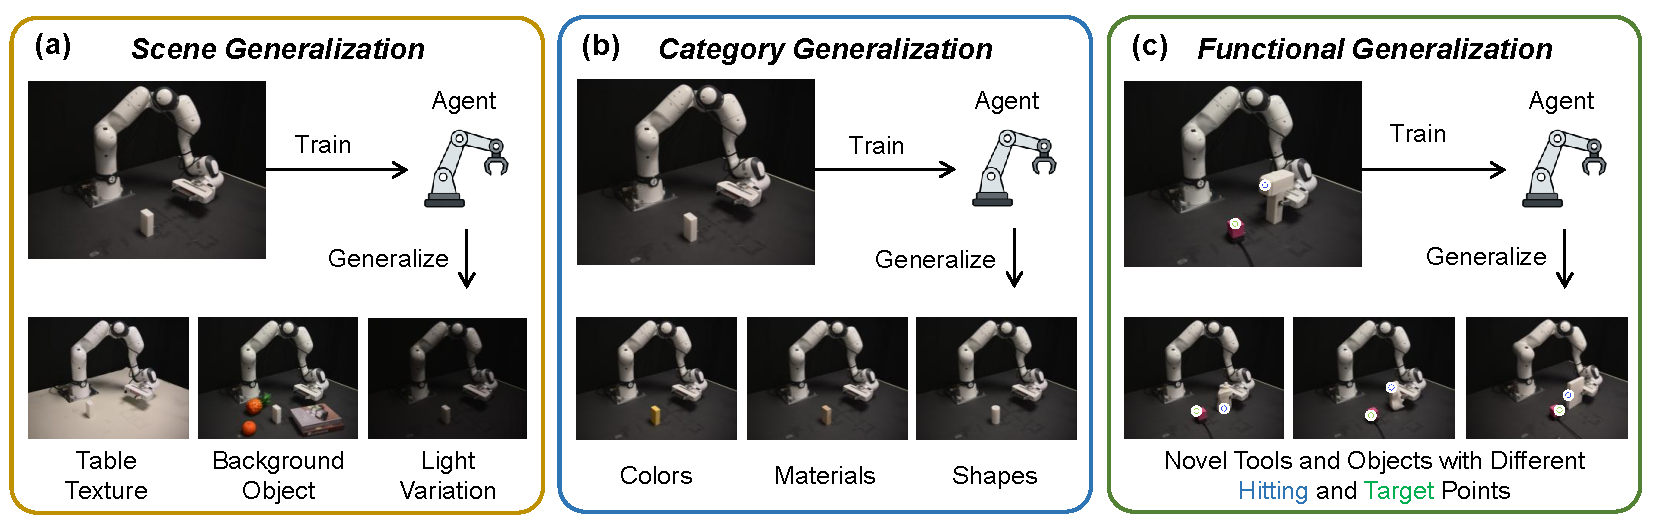
\includegraphics[width=1.0\linewidth]{figures/teaser_v2.pdf}
    \caption{
    \textbf{Comparison between functional generalization and existing generalization settings.}
    (a) Scene generalization evaluates robustness to visual variations.
    (b) Category generalization tests transfer across objects with diverse properties.
    (c) Functional generalization requires using unseen tools to accomplish the same function.
    % (d) The functional intent of hitting.
    }
    \label{fig:functional_generalization}
\end{figure}
Functional generalization is fundamentally harder than conventional generalization. As illustrated in Fig.~\ref{fig:functional_generalization}, scene- and category-level generalization only require tolerating visual variations while the underlying motion stays the same~\cite{goyal2023rvt, shridhar2023perceiver, shridhar2022cliport, nair2023r3m}. Functional generalization, by contrast, demands that the motion itself change: striking a target with a novel tool requires locating its contact region, aligning it, and producing an appropriate motion, even when the tool's shape and trajectory differ entirely from training. The core difficulty is a fundamental mismatch: functionally equivalent tools share recognizable structure in visual space, but this similarity does not transfer to action space, where each tool demands an entirely different motor pattern.


Bridging this perception-to-action gap requires an intermediate representation that carries functional intent across tools, satisfying two competing demands: expressive enough to capture where to make contact and how to move onto the target, yet grounded enough to be predicted from action-free observations without overfitting to tool-specific appearance. Dense representations like raw video entangle function-relevant cues with tool-specific appearance, while overly sparse ones discard the geometric and temporal structure needed for action. This trade-off raises the central question of our work: \textit{which representation best transfers functional intent from perception to action?}

To answer this question, we systematically evaluate intermediate representations 
including affordance images, human video prompts, and 2D keypoint trajectories, 
finding that keypoint trajectories best balance functional expressiveness and 
action groundability: they capture function-relevant contact and motion structure 
while discarding tool-specific appearance that causes overfitting. Building on 
this, we propose \textbf{F}uncti\textbf{O}nal \textbf{R}easoning and 
\textbf{G}rounded \textbf{E}xecution (\algoname{}), a two-stage policy that 
decouples functional reasoning from action execution: it first predicts 
generalizable keypoint trajectories for unseen tools from large-scale action-free 
data, then grounds these functional plans into executable robot actions using a 
small set of action-labeled demonstrations. We further introduce a seven-tool 
hitting-function benchmark, where \algoname{} consistently outperforms 
state-of-the-art methods on unseen tools in both simulation and the real world, 
achieving over $2\times$ improvement in average success rate. In summary, our 
contributions are threefold:
\begin{itemize}[leftmargin=*]
    \item We formalize \textit{functional generalization} in robotic tool-use 
    and identify the perception-to-action gap as its core difficulty.
    \item We find that 2D keypoint trajectories best balance functional 
    expressiveness and action groundability, and propose \algoname{}, a two-stage 
    policy that predicts generalizable keypoint trajectories from action-free data 
    and grounds them into robot actions with limited demonstrations.

    \item Through extensive simulation experiments across seven tools and real-world 
    validation, we demonstrate that \algoname{} consistently outperforms 
    state-of-the-art methods on unseen tools, achieving over $2\times$ improvement in average success rate.

\end{itemize}

% Intuitively, a straightforward method to address this problem is to expose agents to diverse tool-use demonstrations, allowing them to observe how different tools interact with the target over time. However, this strategy faces two key challenges. First, collecting large-scale action-labeled robotic data across diverse tools is time-consuming and labor-intensive, especially for contact-rich tool-use tasks. Additionally, direct visual-to-action learning compresses dense, semantics-rich observations into sparse motor commands, causing function-relevant structures to collapse into tool-specific action patterns. Consequently, the agents tend to overlook transferable cues, such as aligning hitting regions with the same target point, and fail on novel tools. These challenges necessitate a framework that decouples functional intent reasoning from action execution, enabling agents to extract transferable tool-use abstractions and ground them into precise low-level control.

% \lw{
% Bridging this gap requires an intermediate representation that carries the shared affordance from perception into action. 
% Such a representation must satisfy two competing demands. 
% On one hand, it should be \textit{expressive} enough to preserve the function-relevant structure shared across tools, namely, where to make contact and how to bring it onto the target. 
% On the other hand, it should be \textit{groundable}: predictable from action-free observations and decodable into precise actions, without smuggling in tool-specific appearance that the policy would simply overfit. 
% These demands are in tension. 
% Dense representations such as raw video preserve rich detail but entangle function-relevant cues with tool-specific appearance, while overly sparse representations discard the temporal and geometric structure needed to act. 
% This trade-off raises the central question of our work: \textit{which representation best carries affordance similarity from perception to action?}}


% Bridging this gap requires an intermediate representation that carries the shared affordance from perception into action. 
% Such a representation must satisfy two competing demands. 
% On one hand, it should be \textit{expressive} enough to preserve the function-relevant structure shared across tools, namely, where to make contact and how to bring it onto the target. 
% On the other hand, it should be \textit{groundable}: predictable from action-free observations and decodable into precise actions, without smuggling in tool-specific appearance that the policy would simply overfit. 
% These demands are in tension. 
% Dense representations such as raw video preserve rich detail but entangle function-relevant cues with tool-specific appearance, while overly sparse representations discard the temporal and geometric structure needed to act. 
% This trade-off raises the central question of our work: \textit{which representation best carries affordance similarity from perception to action?}


% When humans perform a task such as hitting a nail with an alternative tool, we typically reason about the functional interaction before execution by imagining how the tool may interact with the target, either as a future visual scene or as a possible motion trajectory. Inspired by this process, we aim to explore a functional intermediate representation that bridges dense visual observations and sparse motor commands. An effective representation should be visually predictable from action-free observations, while remaining sufficiently structured to support action grounding. With such a representation, a high-level planner can predict function-relevant future states, and a low-level execution policy can translate them into precise robot actions. This formulation reduces the burden of learning functional intent purely from action-labeled robot data and alleviates the information collapse caused by direct visual-to-action learning.

% In this paper, we propose the Generalizable Functional Plan and Execution (\algoname{}) policy, a System-2/System-1 framework that decouples functional planning from action execution using a functional intermediate representation. We study several candidate representations, including affordance images, human video prompts, and 2D keypoint trajectories, and find that 2D keypoint trajectories provide the best trade-off between visual predictability and action groundability. Our \algoname{} policy therefore trains a System-2 planner to predict future keypoint trajectories as functional plans, and a System-1 execution policy to ground these plans into executable actions. To evaluate functional generalization, we further introduce a hitting-function benchmark across seven tools. Experiments in simulation and real-world settings show that the \algoname{} policy consistently outperforms other state-of-the-art methods on unseen tools.

% \lw{
% To answer this question, we propose \algoname{} (Generalization via Functional Trajectories), a policy built on 2D keypoint trajectories as the functional intermediate representation. 
% Among affordance images, human video prompts, and keypoint trajectories, we find that keypoint trajectories best balance affordance expressiveness and action groundability: they retain the contact point, target, and tool geometry that define the affordance, while discarding the tool-specific appearance that a policy tends to overfit. 
% \algoname{} first predicts future keypoint trajectories from large-scale action-free observations, and then grounds the predicted plan into precise actions using only a small set of action-labeled demonstrations, sidestepping the prohibitive cost of learning functional structure from robot data alone. 
% To evaluate functional generalization, we further introduce a hitting-function benchmark across seven tools, where \algoname{} consistently outperforms state-of-the-art methods on unseen tools in both simulation and the real world, achieving over $2\times$ improvement in average success rate.
% }


% To this end, we propose \textbf{F}uncti\textbf{O}nal \textbf{R}easoning and \textbf{G}rounded \textbf{E}xecution (\algoname{}), a policy built on 2D keypoint trajectories as the functional intermediate representation. 
% Among affordance images, human video prompts, and keypoint trajectories, we find that keypoint trajectories best balance affordance expressiveness and action groundability: they retain the contact point, target, and affordance-relevant tool geometry, while discarding the tool-specific appearance that a policy tends to overfit. 
% \algoname{} first predicts future keypoint trajectories from large-scale action-free data, and then grounds them into actions using a small set of action-labeled demonstrations, sidestepping the prohibitive cost of learning functional structure from robot data alone.
% To evaluate functional generalization, we further introduce a hitting-function benchmark across seven tools, where \algoname{} outperforms state-of-the-art methods on unseen tools in simulation and the real world, achieving over $2\times$ improvement in average success rate. In summary, our contributions are threefold:

% In summary, our contributions are threefold:
% \begin{itemize}[leftmargin=*]
%     \item We identify \textit{functional generalization} as a novel problem in tool-use manipulation, aiming to evaluate whether agents can transfer the same function across diverse and unseen tools.

%     \item \textbf{\algoname{}} policy is proposed as a System-2/System-1 framework that uses 2D keypoint trajectories to bridge functional planning and action execution.

%     \item A 7-tool hitting-function benchmark is developed, where simulation and real-world experiments show that \algoname{} consistently outperforms state-of-the-art methods on unseen tools.
% \end{itemize}

% \lw{
% In summary, our contributions are threefold:
% \begin{itemize}[leftmargin=*]
%     \item We identify \textit{functional generalization} in tool-use manipulation, accomplishing the same function with diverse and unseen tools, and frame its core difficulty as carrying tool affordance from perception to action.
%     \item We find that 2D keypoint trajectories best balance affordance expressiveness and action groundability, and propose \textbf{\algoname{}}, which predicts keypoint trajectories from action-free data and grounds them into actions with limited robot demonstrations.
%     \item We build a seven-tool hitting-function benchmark, where \algoname{} outperforms state-of-the-art methods on unseen tools in both simulation and the real world, with over $2\times$ improvement in average success rate.
% \end{itemize}
% }
% \begin{itemize}[leftmargin=*]
%     \item We identify \textit{functional generalization} in robotic tool-use, completing the same function with unseen tools, and frame its core difficulty as carrying tool affordance from perception to action.
%     \item We find that 2D keypoint trajectories best balance affordance expressiveness and action groundability, and propose \algoname{}, which predicts keypoint trajectories from action-free data and grounds them into actions with limited robotic demonstrations.
%     \item A 7-tool hitting-function benchmark is built, where \algoname{} outperforms state-of-the-art methods on unseen tools in simulation and the real world, with over $2\times$ improvement in success rate.
% \end{itemize}
